
%
% CSC 544 Assignment 7
% 
% @author Benjamin Dicken
% @author Rachel Baumann
%


\documentclass[a4paper, 11pt]{article}
\usepackage{comment} % enables the use of multi-line comments (\ifx \fi) 
\usepackage{fullpage} % changes the margin

\usepackage[english]{babel}
\usepackage[utf8x]{inputenc}
\usepackage{amsmath}
\usepackage{graphicx}
\usepackage{mathtools}
\usepackage{hyperref}
\usepackage{latexsym}
\usepackage{amssymb}
\usepackage{amsfonts}
\usepackage{amstext}
\usepackage{multicol}
\usepackage{amsxtra} 
\usepackage[margin=0.7in]{geometry}
\usepackage{algorithm2e}
\usepackage{framed}
\usepackage{booktabs}


\title{CSc 544 Assignment 7}
\author{Benjamin Dicken and Rachel Baumann}

\begin{document}
\maketitle
\noindent

\section*{The Dataset}

%Description of the data set we're using goes here...
%
%colors.csv
%pieces.csv
%sets.csv
%set\_pieces.csv
%
%images:
%parts
%sets

We are using a dataset from \href{http://rebrickable.com/}{Rebrickable.com} on the inventories of every official LEGO set up to 2015. This dataset includes 9,992 lego sets, 21,089 unique pieces in 130 colors, with a total of 479,751 relations between the sets and pieces. This dataset also includes images of 9,457 of the sets and most of the pieces. All data for the sets, pieces, colors, and maps between the pieces and sets are stored in csv files and the images are jpeg files. We have the following information in the fours csv files:

\begin{enumerate}

\item {\bf Sets:} Includes an ID for each set, the year a set was released, the total number of pieces in a set, and a category and brief description for each set.

\item {\bf Pieces:} Includes an ID, category and brief description for each piece.

\item {\bf Set Pieces:} Includes a set and piece ID, the number of times the piece is used in the set, the color of the piece in the set, and whether the piece is a normal or spare piece.


\item {\bf Colors:} Includes an ID and a brief description for each color.

\end{enumerate}



\section*{Investigation of the Dataset and Results}

We have spent the past several weeks writing scripts to fetch the LEGO data and images, exploring the data, and experimenting with several types of visualizations.

Downloading the data was a relatively straightforward process. All of the information for sets, pieces, colors, and the mapping between sets and pieces came as well-organized csv files packed into a single zip file. All we had to do was extract the data from the zip. The piece images also came bundled in zip files. Getting the images for the sets was a little trickier. \texttt{rebrickable.com} does not distribute those images in an easy-to-download format. To get the images, we wrote a simple web-scraper (in \texttt{bash}) which crawled \texttt{rebrickable.com} for all the images.

The next step was to explore the data, and ensure that it behaved as expected. We wrote a simple web interface to browse all of the sets, pieces, and the mapping between them. We discovered that most of the data was in-tact and well-organized, so it needed very little cleaning. The oly issue we ran into was a few missing piece and set images, but this was minor.

Once we were confident that the data was clean, we began experimenting with a few basic visualization techniques. We started off by making many simple scatterplots to get a feel for the many dimentions of the data. After going through this process, we got a good feel for what we had, and what we didn't. See some scatterplots we tried in figure 1.

\begin{figure}[h!]
\centering
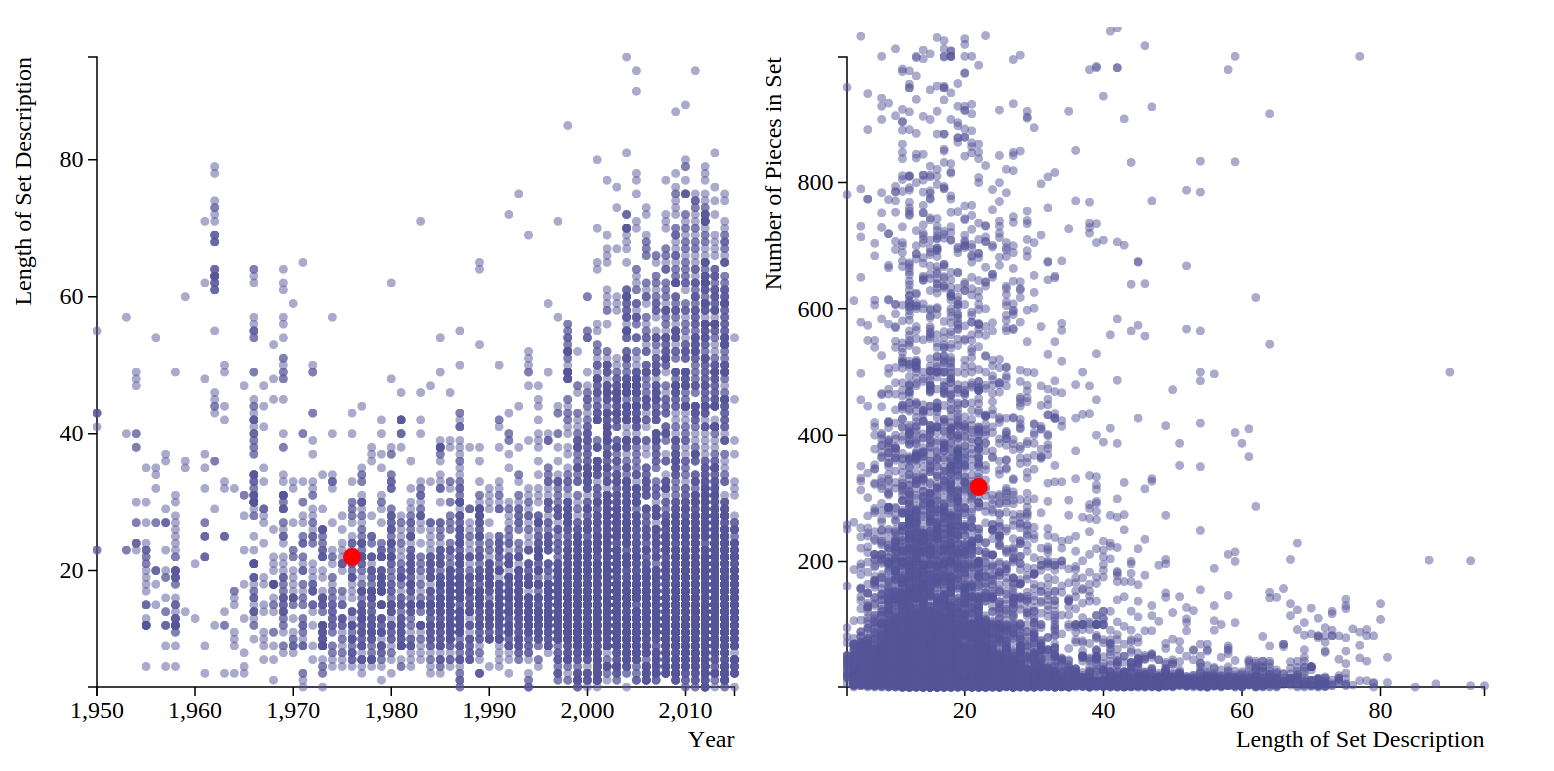
\includegraphics[width=0.8\textwidth]{img/scatterplots.png}
\caption{Two of many scatterplots we experimented with.}

\end{figure}

We then decided to try plotting all of the LEGO sets onto a single plane, using the t-SNE algorithm. For the vector of similiarties, which t-SNE requires to be creatd for each node on the graph, we used a simple binary similarity function. First, we computed the set $t1$ of all the individual tokens in the descriptions of all the sets and pieces that occur more than $n$ amount of times (where $n$ is some threshold). Next we computed a set of description tokens for each lego set, using all the tokens found in the set's description and the description of all it's pieces. For each token $t$ in $si$, we add a number to the similarity vector. We add a 9 if $t \in$ the LEGO set's token set, and a $1$ if it does not. Each set, along with it's computed similarity vector, is passed along to the t-SNE algorithm and visualized.

After quite a bit of fine-tuning, we got the t-SNE layout looking nice. We plan on using the t-SNE layout, several scatterplots, and potentially a few other simple visualizations in combination in our final product.


\section*{Project Goal for Visualization}

We are currently working on linking the t-SNE visualization of all the LEGO sets with a collection of scatterplots summarizing the information from the collection of all the data on the LEGO sets. At present we have the ability to zoom in on the t-SNE graph and would like to connect it to at most 6 visible scatterplots off to one side of the visualization. At present we are working to develop a better labeling system on  the t-SNE graph so that the visualization doesn't show labels for all the sets in the global view. Our plan is to only display the categories of the sets on the global view of t-SNE. These labels  will be place on the average of the coordinates of all sets with the matching category. 
However, once zoomed in far enough a brief description of each set will appear on the t-SNE graph providing the user with more specifics on the zoomed in sets.  \\

Next, we would like to connect both the t-SNE graph and scatterplots with brushes to allow the user to filtering the data on any of the scatterplots or on the t-SNE graph. Any brushing will then be reflected on all the scatterplots and on the t-SNE graph. 
 We are currently showing details on demand by allowing the user to select a point on any scatterplot, which is then highlighted on all scatterplots and reveals a table of information for the selected set. In the future, this will also be connected to the t-SNE graph to allow the user to select a set there and see the table and set highlighted on all scatterplots.

\end{document}
